%\usepackage{physics}
\section{That Kepler boy and his weird circles}
    
    \frame{\sectionpage}
    
    \begin{frame}{The Laws of Kepler}
    \begin{enumerate}
        \uncover<+->{\item The orbits of planets around the sun are in ellipses, with the Sun at one of the focii}
        
        \uncover<+->{\item The areal velocity of the planet is a constant}
        
        \uncover<+->{
            \item The square of the period of orbit of the planet in years is equal to the cube of the semi-major axis of the orbit in AU}
    \end{enumerate}
    \end{frame}
    
     \begin{frame}
         \begin{figure}
             \centering
             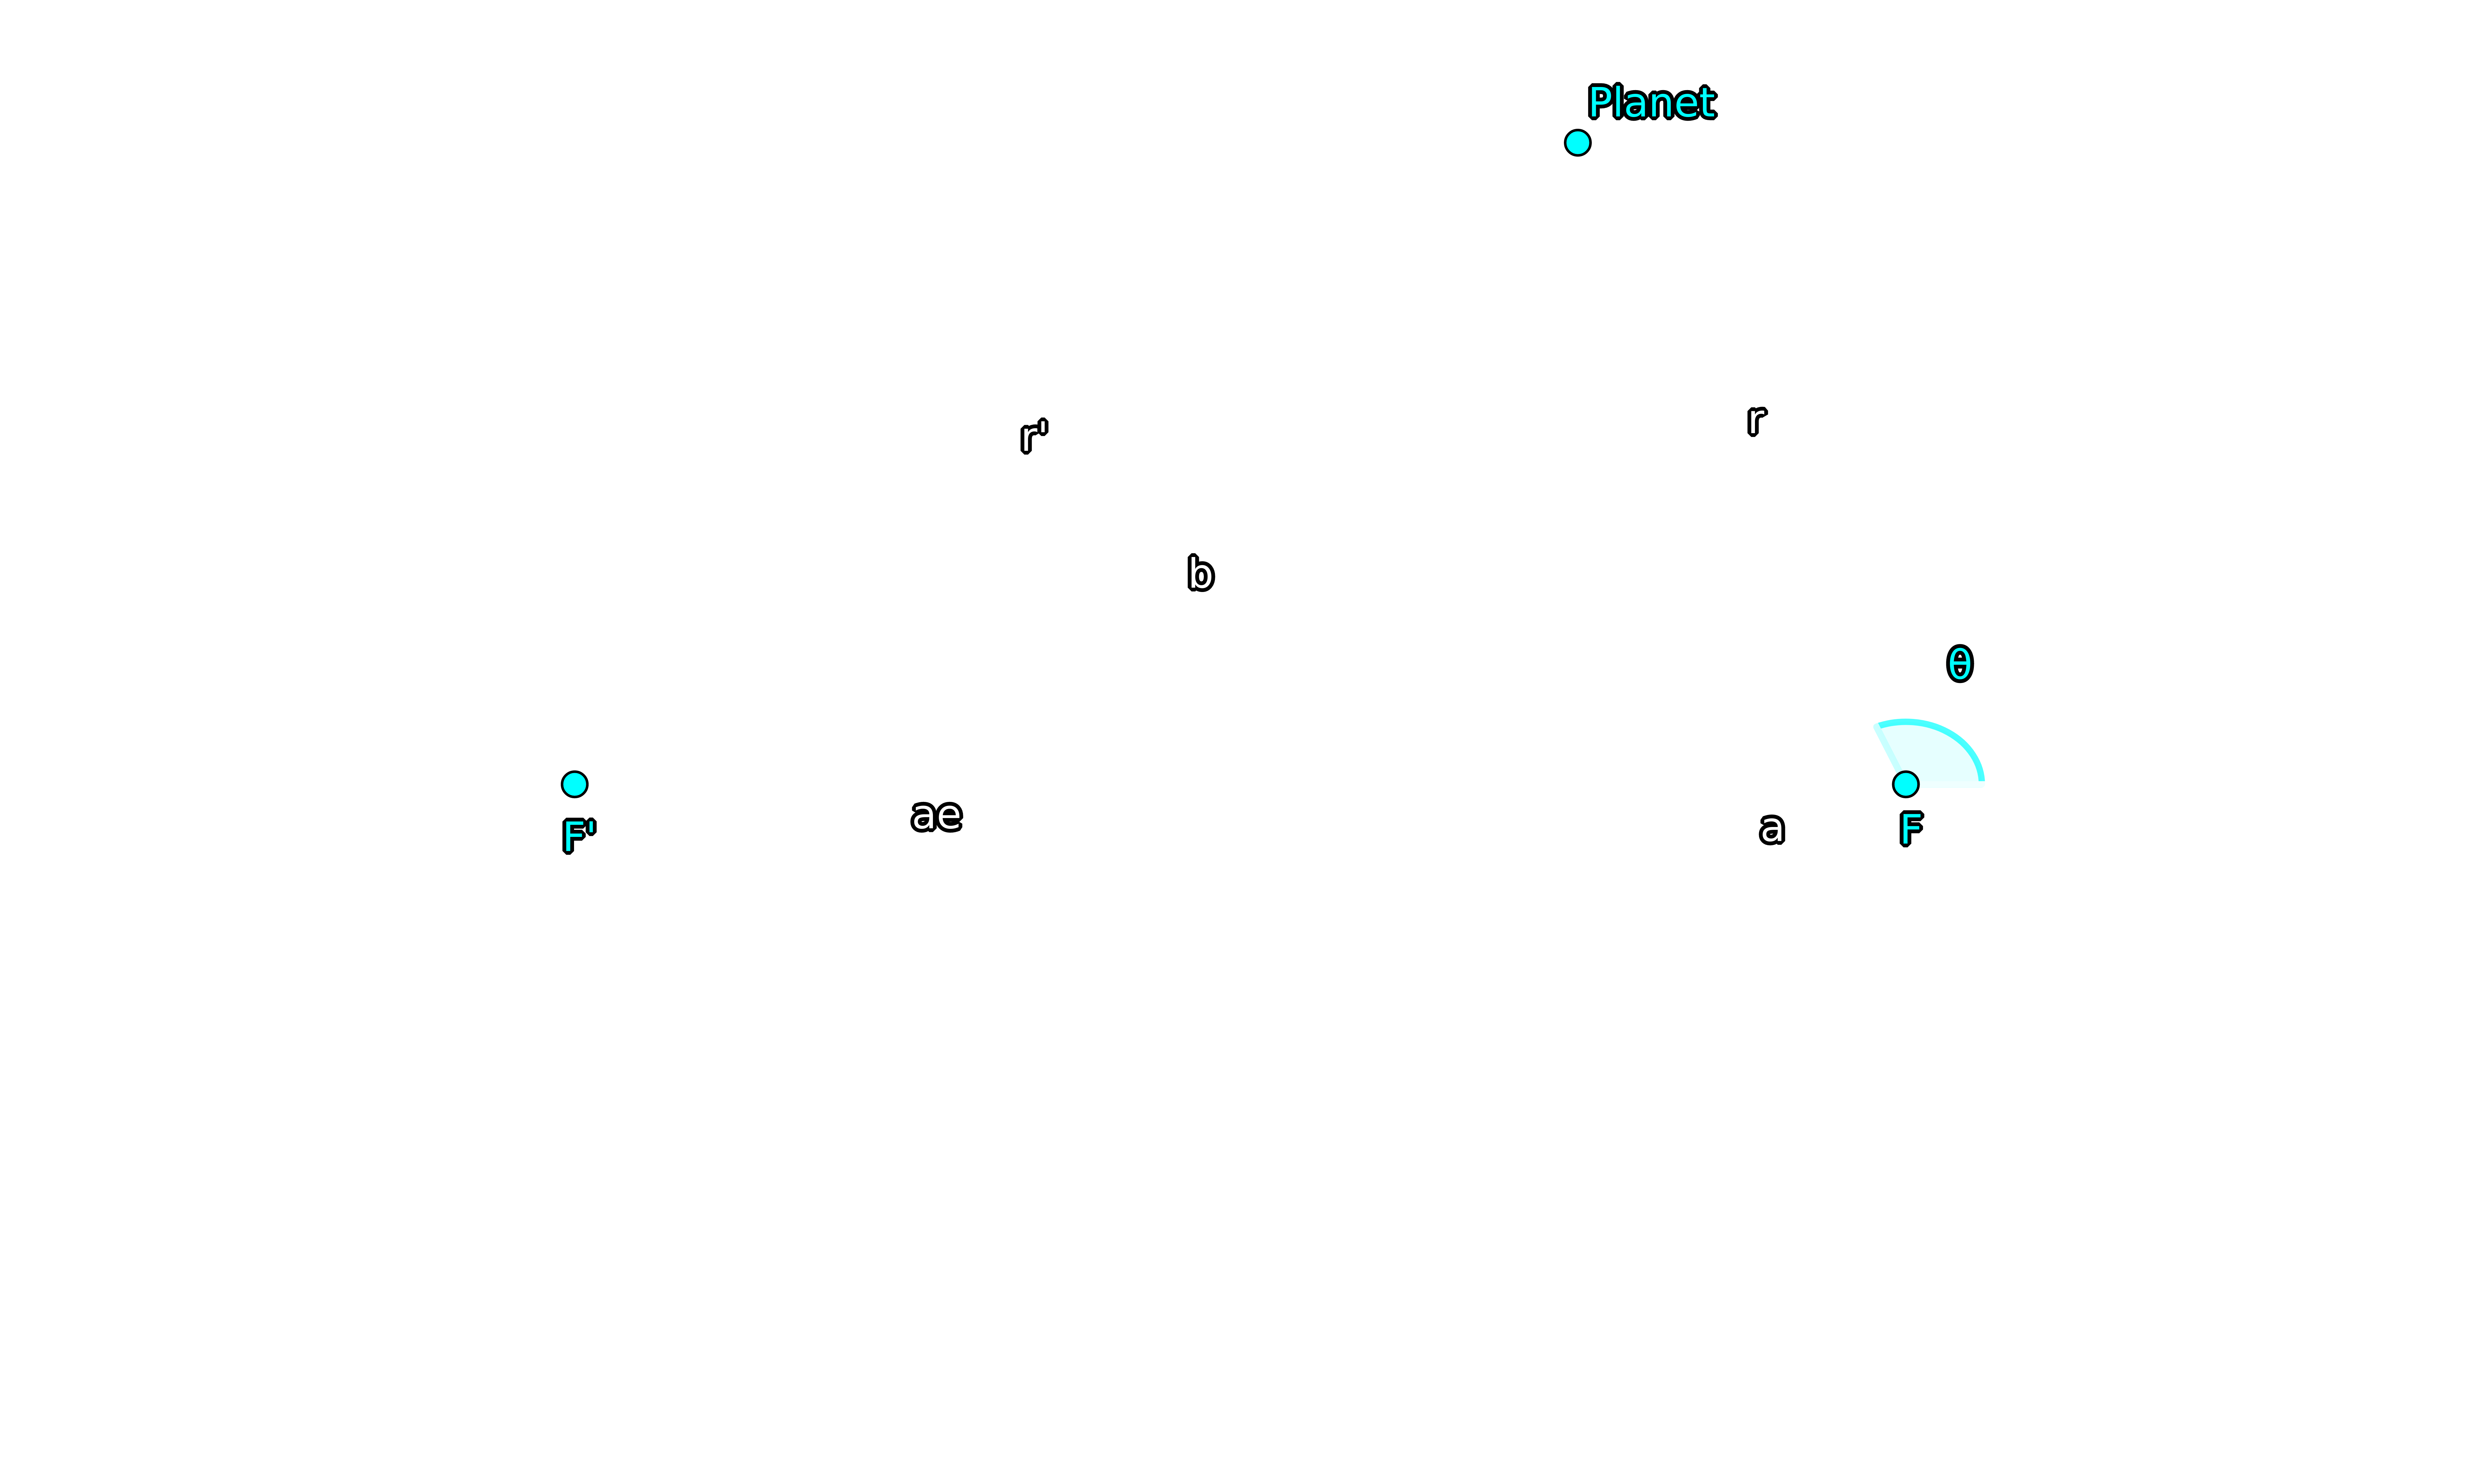
\includegraphics[width=\textwidth]{images/elliptical_orbit.png}
             \caption{Orbit of a planet}
             \label{fig:Orbit_ellpise}
         \end{figure}
     \end{frame}
    
    \begin{frame}{The Laws of Kepler Reloaded}
        \uncover<+->{\begin{equation}
        \label{ellipse_eqn}
            r = \frac{a(1-e^2)}{1 + e\cos \theta}
        \end{equation}}
        \uncover<+->{
        \begin{equation}
        \label{ang_mom_cons}
            r^2 \dv{\theta}{t} = {\rm constant}
        \end{equation}}
        \uncover<+->{
        \begin{equation*}
            P^2\ ({\rm in\ years}) = a^3\ ({\rm in\ AU})
        \end{equation*}}
    \end{frame}
    
    \begin{frame}{The Laws of Kepler Revolutions}
        \begin{equation}
            \vb{F} = -\frac{Gm_1m_2}{r^2}\vu{r}
            \label{NewtonsLaw}
        \end{equation}
        
    \end{frame}
	
	\subsection{Motivating Newton's Law}
	\frame{\sectionpage}
	\begin{frame}{Standing on the shoulders of giants (so not Hooke)}
		This is relatively simple to do with calculus
	\end{frame}
	
	\begin{frame}
	In plane polar co-ordinates, we have
	$$\vb{r}=r \hat{\vb{r}}$$
	$$\dot{\vb{r}}=\dot{r}\hat{\vb{r}}+r\dot{\theta}\hat{\bm{\theta}}$$
	$$\ddot{\vb{r}}=(\ddot{r}-r\dot{\theta}^2)\hat{\vb{r}}+(2\dot{r}\dot{\theta}+r\ddot{\theta})\hat{\bm{\theta}}$$
	That last term in the third equation looks familiar. 
	$ r^2 \dot{\theta} ={\rm constant }\implies 2r\dot{r}\dot{\theta} + r^2 \ddot{\theta} = 0$, so immediately, Kepler's second law implies that the gravitational force is radial (apart from the obvious(?) conservation law)
	
\end{frame}
	
	\begin{frame}
		Kepler's first law gives us
		$$r = \frac{a(1-e^2)}{1 + e\cos \theta}$$
		Differentiating with respect to time,
		$$\dot{r}=-\frac{l}{(1-e\cos{\theta})^2}e\sin{\theta}\;\dot{\theta}$$
		Now, we can use Kepler's second law ($\dot{A}=\frac{1}{2}r^2\dot{\theta}=k$) and substitute $\dot{\theta}$ in terms of $r$ and put back Kepler's first law to substitute for the $(1-e\cos{\theta})$ term in the denominator to eventually get
		$$\dot{r}=-\frac{2k}{l}e\sin{\theta}$$
		and differentiating again and simplifying as above, we get
		$$\ddot{r}=-\frac{4k}{l r^2}\left(1-\frac{l}{r} \right)$$
	\end{frame}
	
	\begin{frame}
		Now, we can write the acceleration $\ddot{\bm{r}}$ as
		$$\ddot{\bm{r}}=\left[-\frac{4k}{l r^2}\left(1-\frac{l}{r} \right)-r\left(\frac{2k}{l} \right)^2\right]\hat{\bm{r}} = -\frac{4k}{l r^2}\hat{\bm{r}}$$
		So, we get the force to be of the form, 
		$$\bm{F}=m\ddot{\bm{r}}=-\frac{4 m k/l}{r^2}\hat{\bm{r}}$$
	\end{frame}
	
	\begin{frame}{But wait...}
		\onslide*<1->{We have more: the planet's frame of motion. \\The same calculation will yield the same results, with the masses exchanged.}
		\\[3\baselineskip]
		\onslide+<2->{Confused?}
	\end{frame}
	\begin{frame}
		\begin{figure}
			\centering
			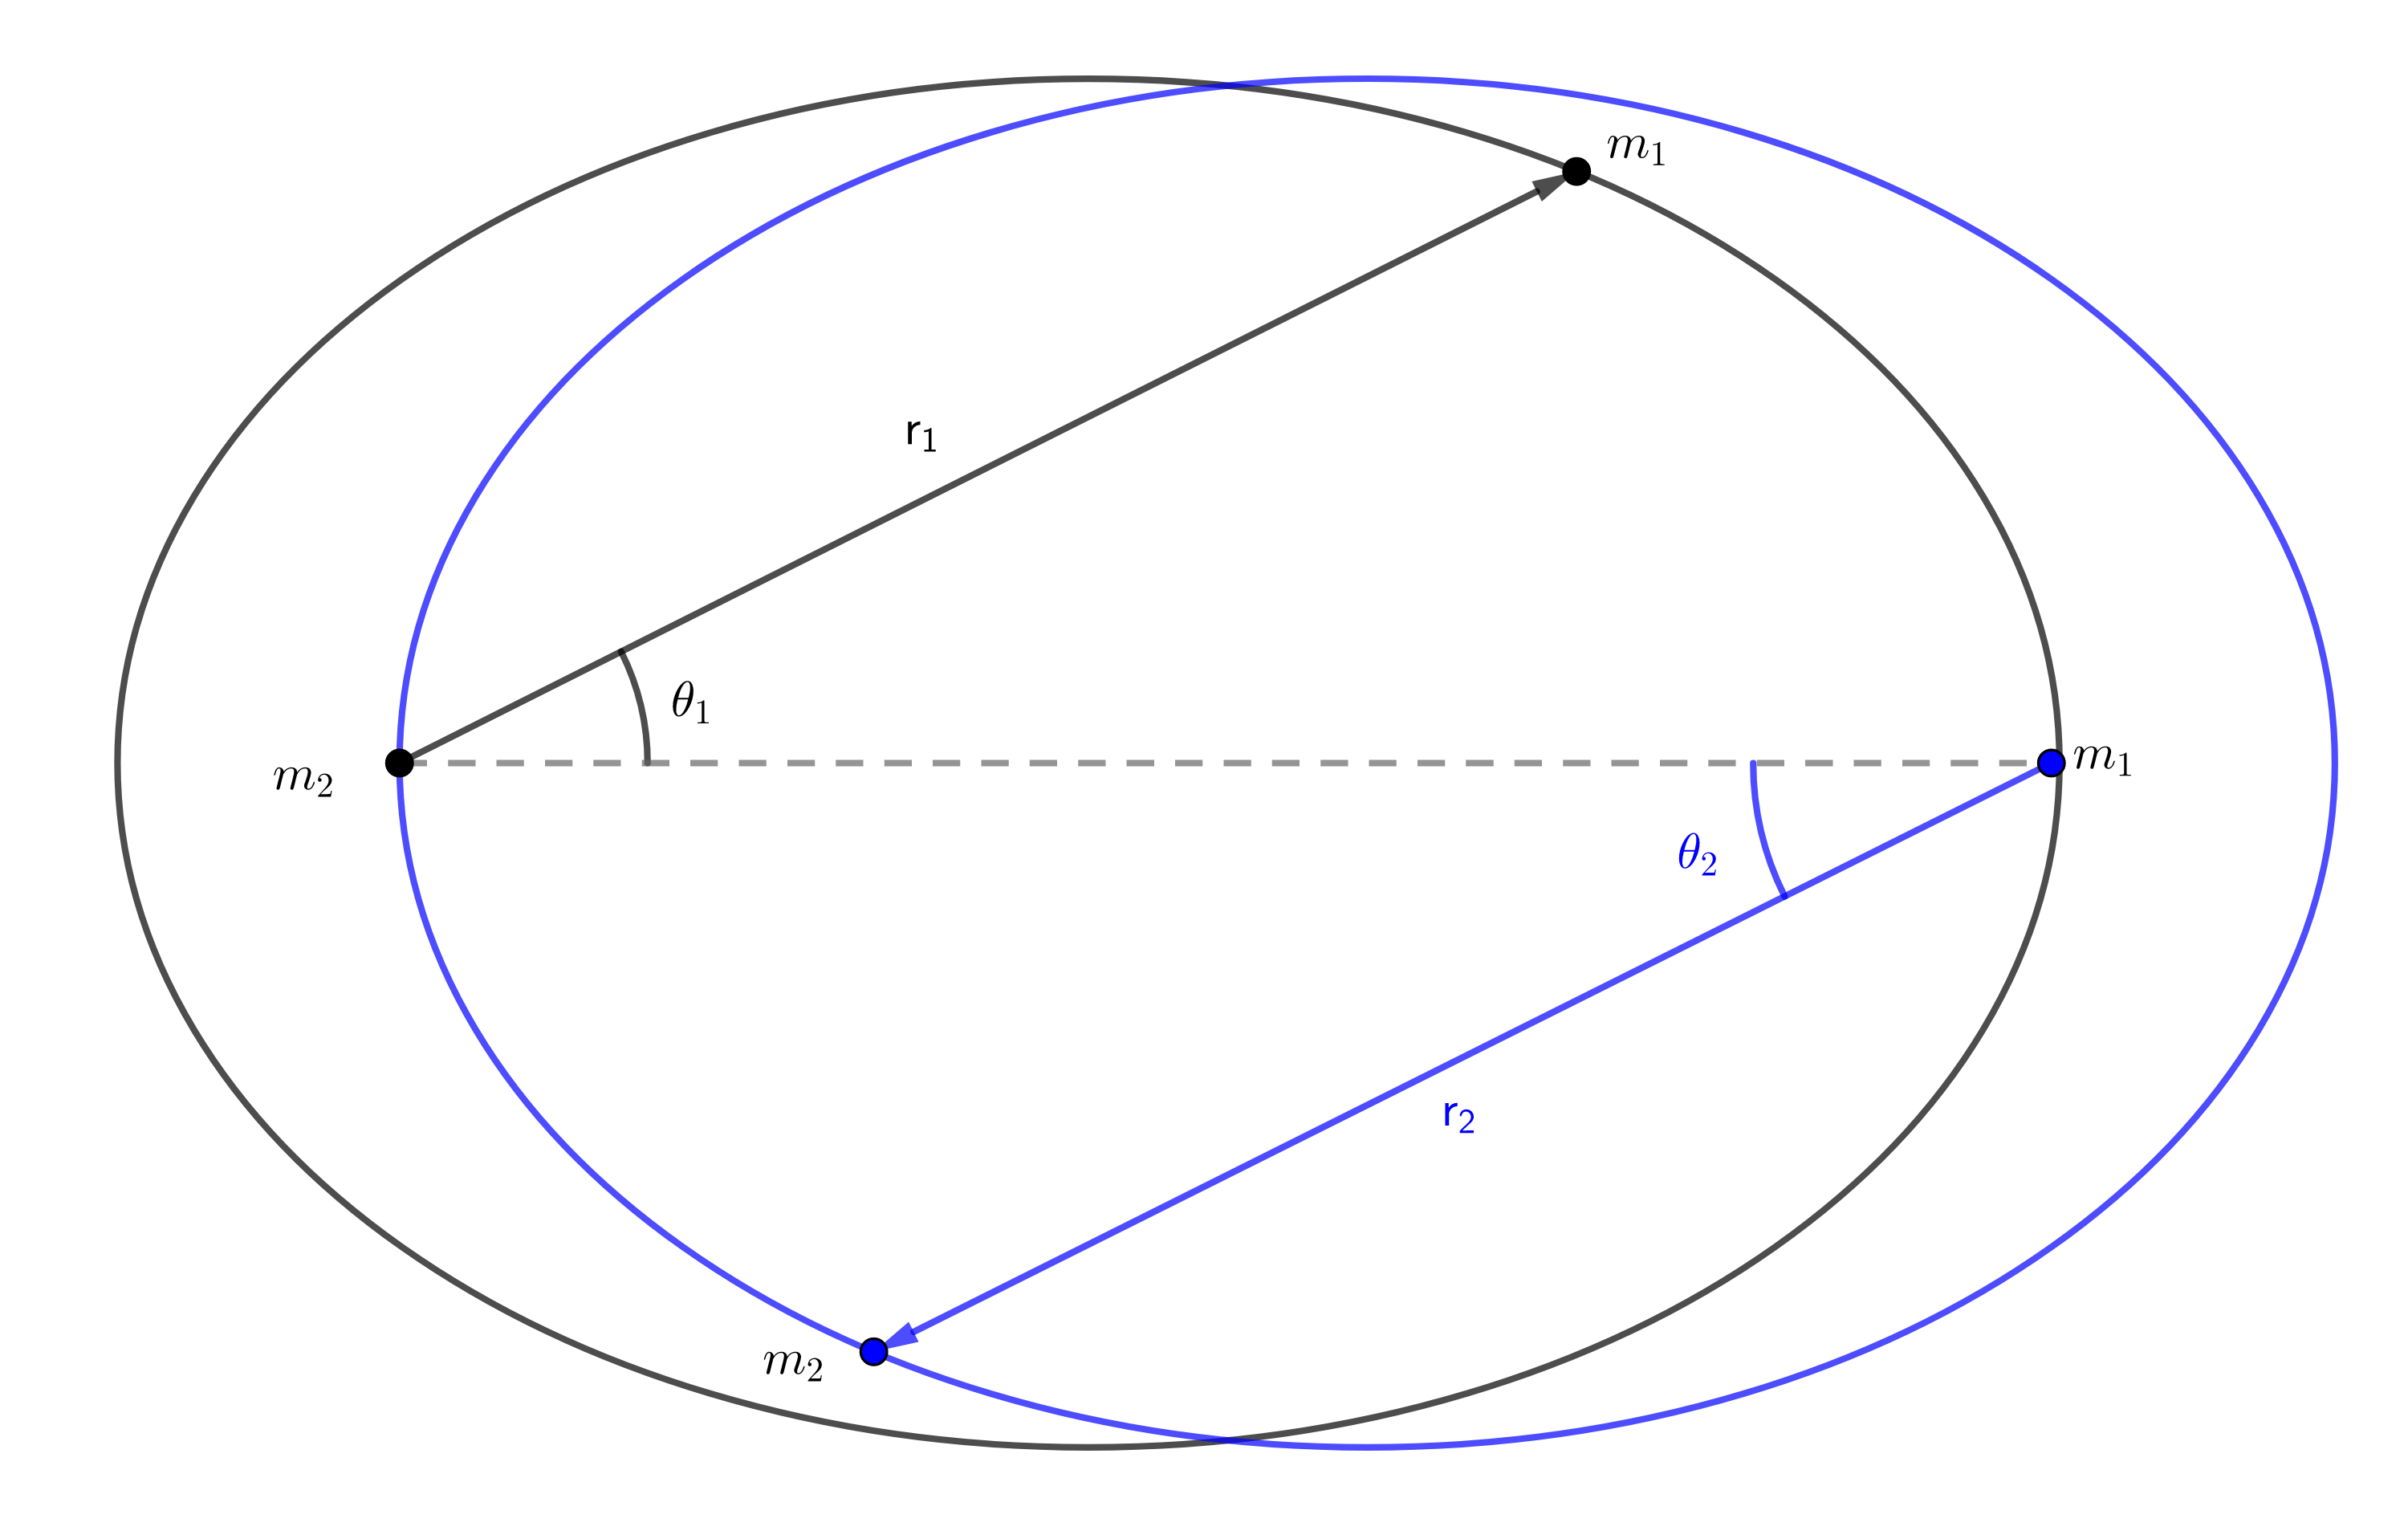
\includegraphics[width=\textwidth]{images/different_frames.png}
		\end{figure}
	\end{frame}

	\begin{frame}
		From the frame of $m_1$, we can write the force $\bm{F}_{12}$ exerted by $m_1$ on $m_2$ as
		$$\bm{F}_{12}=-\frac{4m_2 k_1}{l r_1^2}\hat{r_1}$$
		and conversely,
		$$\bm{F}_{21}=-\frac{4m_1 k_2}{l r_2^2}\hat{r_2}$$
		\newpage
		Now, using Newton's Third Law, and accounting for the fact that $r_1=r_2$ and $\hat{\bm{r}_1}=-\hat{\bm{r}_2}$, we get
		$$\bm{F}_{12}=-\bm{F}_{21}$$
		$$m_1 k_1=m_2 k_2$$
		i.e.
		$$\frac{k_1}{k_2}=\frac{m_2}{m_1}=\alpha$$
		$\alpha$ is a constant with respect to mass of the bodies, the distance between them and time. So, we can write the force as 
		$$\bm{F}_{12}=-\frac{4\alpha m_1 m_2}{r^2}\hat{\bm{r}}$$
	\end{frame}

	\begin{frame}
		This should make it obvious why Newton's Law looks the way that it does. 
		\begin{equation}
			\vb{F} = -\frac{Gm_1m_2}{r^2}\vu{r}
		\end{equation}
	\end{frame}
	
	
	
	